I en klasse D forsterker fungerer transistorene som brytere, de er enten av
eller på.
Bryterne er vanligvis MOSFET transistorer men kan også være vakuumrør eller BPJ.



\paragraph{Virkemåte} \mbox{} \\
Et analogt signal konverteres til pulser ved f.eks. PWM (pulse width
modulation).
\\\\
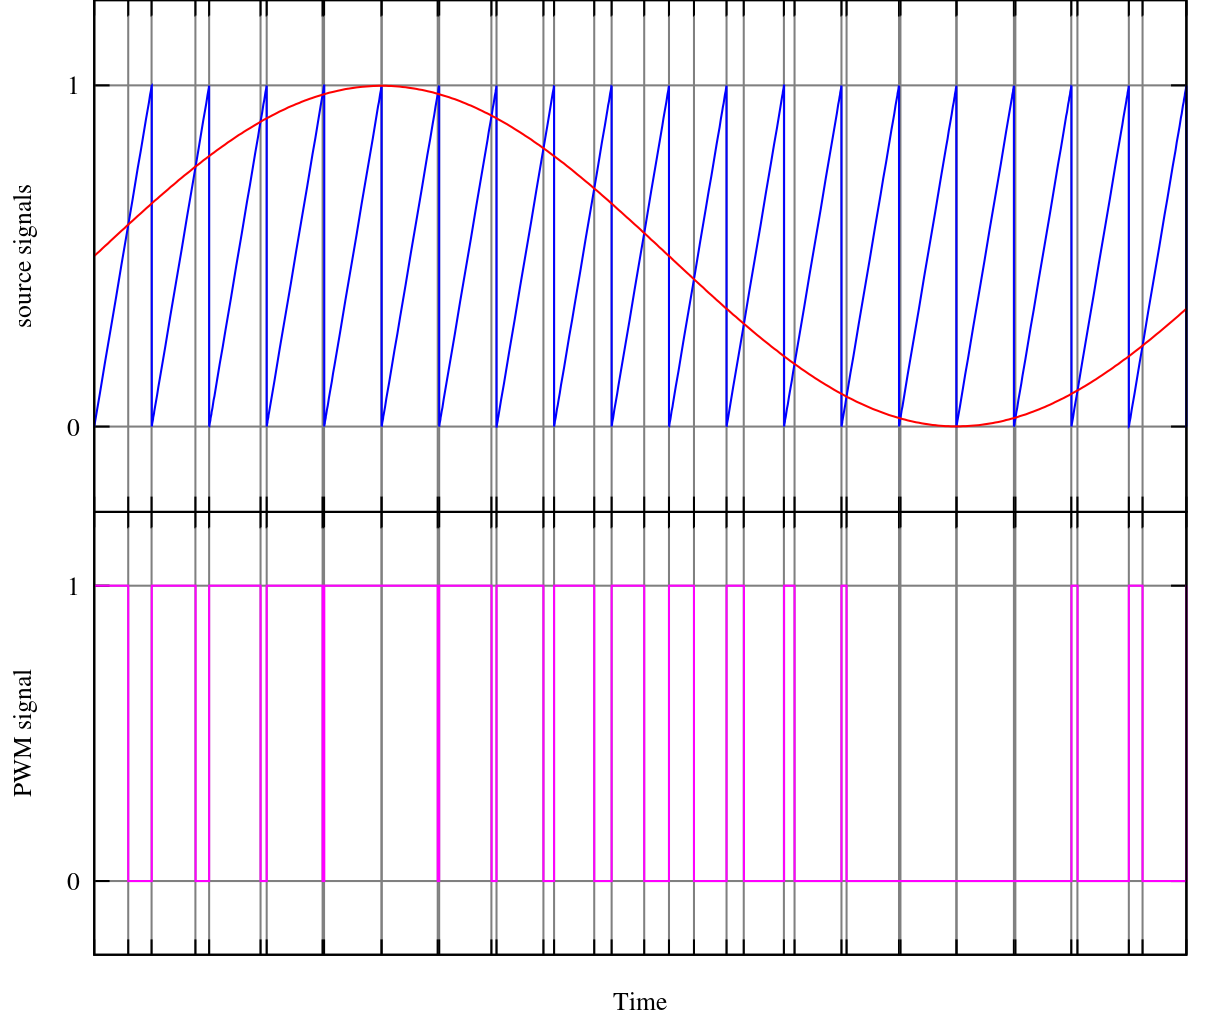
\includegraphics[width=\textwidth]{./img/pwm}
\\\\
Den blå sagtannbølgen er klokkesignalet. \\
Den røde sinusbølgen er signalet som skal moduleres. \\
Den rosa pulsen er signalet etter moduleringen. \\
\\
Når klokka er sterkere enn kilden, brytes pwm signalet.
Men når klokka er svakere enn kilden, er pwm positiv.



\paragraph{Forsterkning} \mbox{} \\
Det analoge signalet kan oversettes til pulser, pulsene forsterkes og
så oversettes signalet tilbake til analogt.
\\\\
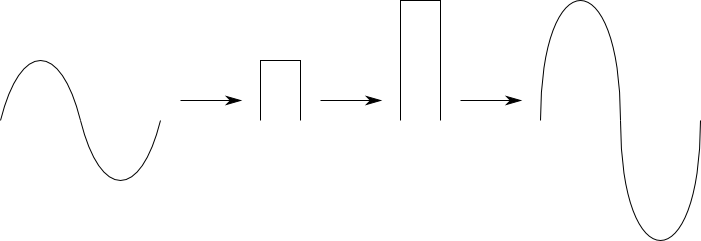
\includegraphics[width=\textwidth]{./img/Damp}
